\documentclass[11pt]{article}
\usepackage[margin=0.7in]{geometry}
\usepackage{graphicx,booktabs,tabularx,array}
\usepackage{titlesec}
\setlength{\parskip}{5pt}
\setlength{\parindent}{0pt}
\titleformat{\section}{\large\bfseries}{}{0pt}{}
\begin{document}
\begin{center}
{\LARGE Group 88 - UDL Assignment 2: Part C}\\[3pt]
{\large Comparative Analysis: beta-VAE, VQ-VAE + PixelCNN, WGAN and WGAN-GP}\\[6pt]
CIFAR-10 | PyTorch | Standard Inception FID on 5,000 real and generated images
\end{center}

\section*{Evaluation summary}
\begin{center}
\begin{tabular}{lrrr}
\toprule
Model & Reconstruction PSNR (dB) & Standard FID $\downarrow$ & Training (min)\\
\midrule
beta-VAE ($\beta$=1) & 18.02 & 200.98 & 4.64\\
VQ-VAE + PixelCNN (K=256) & 24.20 & 150.42 & 12.15\\
WGAN & N/A & 168.33 & 8.31\\
WGAN-GP & N/A & 158.47 & 14.08\\
\bottomrule
\end{tabular}
\end{center}

\section*{Comparative discussion}
\textbf{Reconstruction error.} PSNR is meaningful only where an input image is reconstructed. VQ-VAE (K=256) achieved 24.20 dB, clearly above beta-VAE ($\beta$=1) at 18.02 dB, so it produced lower pixel reconstruction error. Among all VQ codebooks, K=512 had the best reconstruction PSNR (24.77 dB); K=256 is retained here because the assignment specifies it for the Part C visual comparison.

\textbf{Sampling quality.} Standard Inception FID compares distributions of unpaired real and generated images, so it is appropriate for every model. VQ-VAE + PixelCNN (K=256) had the best Part C FID (150.42). WGAN-GP improved on WGAN (158.47 versus 168.33), supporting the expected benefit of gradient penalty over weight clipping. For beta-VAE, increasing beta degraded FID: beta=1 was 200.98, beta=2 was 244.29, beta=4 was 276.73, and beta=10 was 313.46. Within the VQ sweep, K=128 had the lowest FID (139.33), showing that the FID/reconstruction trade-off should be discussed rather than assuming the highest PSNR setting is best for samples.

\textbf{Speed.} beta-VAE was fastest at 4.64 minutes per run because it trains one encoder-decoder model. VQ-VAE + PixelCNN took 12.15 minutes because it trains the VQ-VAE, extracts discrete latents, and trains an autoregressive prior. WGAN took 8.31 minutes; WGAN-GP was slowest at 14.08 minutes because its gradient penalty adds differentiation work during critic updates.

\textbf{Conclusion.} VQ-VAE gave the strongest reconstruction result for the required K=256 comparison and the best Part C FID. WGAN-GP was the stronger GAN variant, at a higher compute cost. PSNR is deliberately marked N/A for GANs because they have no paired reconstruction target.

\newpage
\section*{100 visual examples per model}
\begin{center}\textbf{beta-VAE ($\beta$=1) reconstructions}\\[3pt]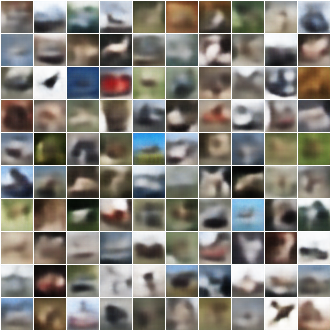
\includegraphics[width=0.82\textwidth]{beta_vae.png}\end{center}
\newpage
\begin{center}\textbf{VQ-VAE + PixelCNN (K=256) samples}\\[3pt]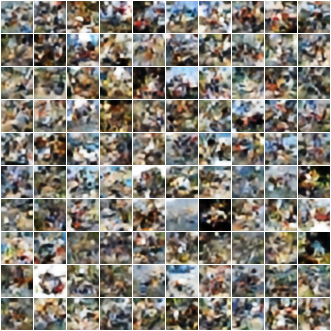
\includegraphics[width=0.82\textwidth]{vq_vae.png}\end{center}
\newpage
\begin{center}\textbf{WGAN samples}\\[3pt]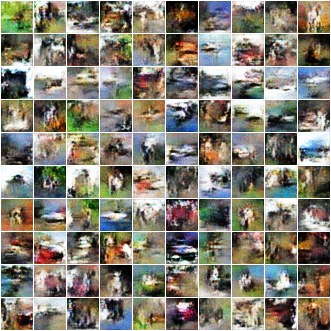
\includegraphics[width=0.82\textwidth]{wgan.png}\end{center}
\newpage
\begin{center}\textbf{WGAN-GP samples}\\[3pt]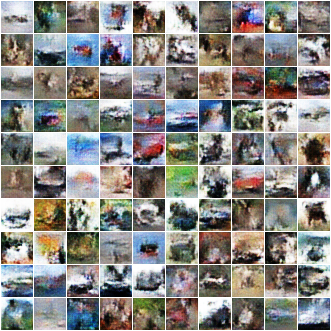
\includegraphics[width=0.82\textwidth]{wgan_gp.png}\end{center}
\end{document}
